\subsection{Architecture}

Our product it made up of two parts: the control server, and the door nodes.
Our product interacts with two types of actors: Operators and Users.

The control server maintains a database of operator profiles, operator logs,
user profiles, and interaction logs.  The control server will use the operator
profiles to validate users using the operator GUI.  Every action performed in
the operator GUI will be logged in the operator logs.  Operators can create and
modify user profiles.  When a user attempts to use a door node, their identity
is checked against their user profile.  Each interaction with a door node is
recorded in a user log.

\begin{figure}[!htb]
\centering
\includegraphics[width=\textwidth]{uml/architecture.png}
\caption{UML Architecture Diagram}
\label{fig:architecture-diagram}
\end{figure}

\subsection{Communication Protocol}

\begin{itemize}
\item Account ID: (number) uniquely identifies an account
\item Node ID: (number) uniquely identifies a door node
\item Transaction ID: (number) uniquely identifies a transaction
\item Current time: (number) Time message was sent
\item Information Request: (list of keys) A list of information required to further the
transaction
\item Information Response: (list of key value pairs) Contains obtained information
\item Access Request Response: (boolean)
\end{itemize}

\begin{table*}[htb]
\begin{tabular}{ l | l | l | p{4.5cm} }
\toprule
Sender & Receiver & Message & Data Format\\
\midrule
Door Node & Control Server & ACCESS\_REQUEST &
Node ID \newline Transaction ID \newline Current time \newline Account ID\\
\hline
Door Node & Control Server & INFORMATION\_RESPONSE &
Node ID \newline Transaction ID \newline Current time \newline Information Response\\
\hline
Control Server & Door Node & INFORMATION\_REQUEST &
Node ID \newline Transaction ID \newline Current time \newline Information Request\\
\hline
Control Server & Door Node & ACCESS\_RESPONSE &
Node ID \newline Transaction ID \newline Current time \newline Account ID \newline Access Request Response\\
\bottomrule
\end{tabular}
\caption{Messages}
\end{table*}

\subsection{Message Sequence Diagrams}

As seen in Figure \ref{fig:message-sequence-diagram}, all message sequences are
initiated by the Door Node sending an ACCESS\_REQUEST.  The Control Server can
reply with an ACCESS\_RESPONSE to immediately grant or deny access.  If the
Control Server doesn't have enough information to make a decision, it will send
INFORMATION\_REQUEST's until it has enough information to send an
ACCESS\_RESPONSE message.

These messages are built in a way that additional sensors could easily be added
to system.

Since there are separate Door Nodes for entrances and exits, the Control Server
can determine if a user is entering or exiting based on the Node ID.  If a Door
Node is to be used for both entering and exiting, it will be equipped with two
NFC Security Badge Readers.  The Door Node will use a separate Node ID for
interactions with each NFC Security Badge Reader.  The Control Server will view
this Door Node with two NFC Security Badge Readers as two separate Door Nodes.

When a user is entering the building, the Control Server will consult the
database to determine if the user is authorized to enter the building.  If the
the user is not authorized, the Control Server will respond with an
ACCESS\_RESPONSE message denying the user.  If the user is authorized, the
Control Server will respond with an INFORMATION\_REQUEST for the user's
temperature.  The door node will then respond with an INFORMATION\_RESPONSE
containing the user's temperature.  The Control Server will repeat the
INFORMATION\_REQUEST for temperature until a temperature not indicating a fever
is received, or the maximum number of tries is reached.  The Control Server
will then respond with an ACCESS\_RESPONSE message denying the user if it is
determined they might have a fever or granting access to the user if their
temperature is normal.  The Control server will then update the database.

When a user is exiting the building, the Control Server will immediately respond
with an ACCESS\_RESPONSE message granting access to the user.  The Control
Server will then use this information to update the database.

\begin{figure}[!htb]
\centering
\includegraphics[width=\textwidth]{uml/message-sequence-diagram.png}
\caption{Message Sequence Diagram}
\label{fig:message-sequence-diagram}
\end{figure}

\subsection{Database Schema}

\begin{figure}[!htb]
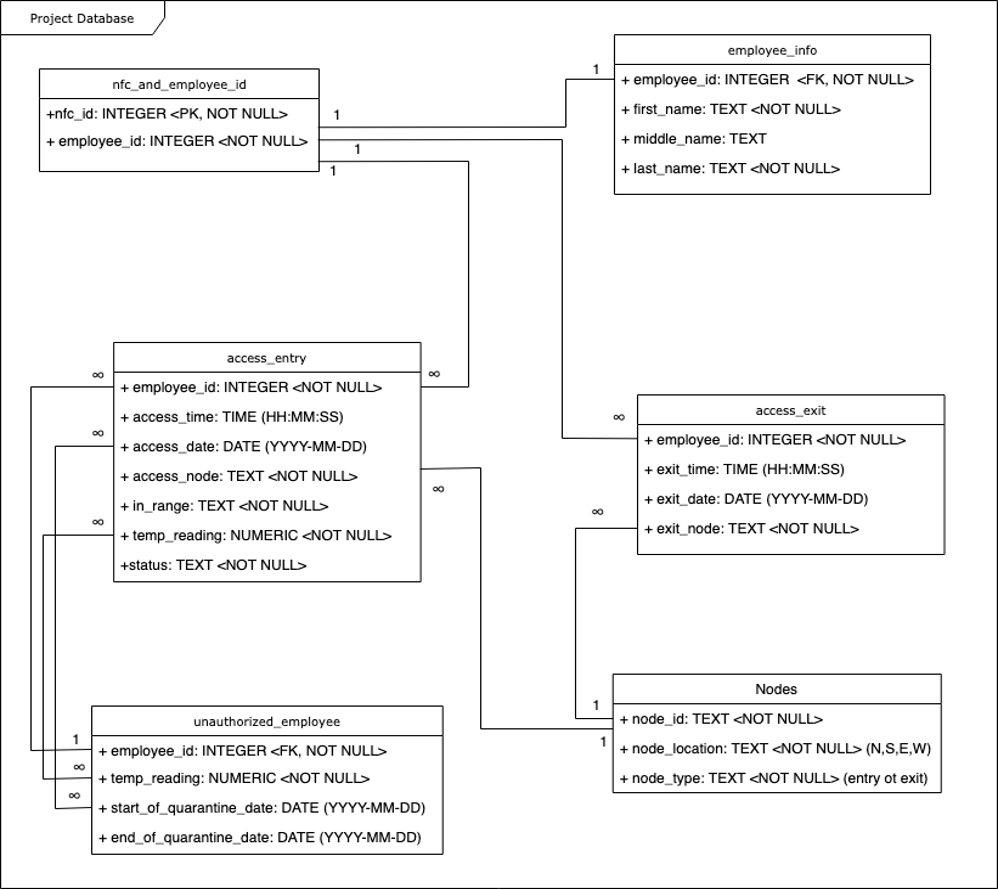
\includegraphics[width=\textwidth]{images/db-schema.png}
\caption{Database Schema}
\end{figure}

